\documentclass[sigchi,nonacm]{acmart}

\def\BibTeX{{\rm B\kern-.05em{\sc i\kern-.025em b}\kern-.08emT\kern-.1667em\lower.7ex\hbox{E}\kern-.125emX}}

\usepackage[utf8]{inputenc}
\usepackage{booktabs}
\usepackage{stfloats}
\usepackage{subcaption}
\usepackage{caption}
\usepackage{graphicx}
\usepackage{placeins}
\usepackage{multicol}
\usepackage{multirow}
\usepackage{hyperref}
\usepackage{fontawesome5}

\copyrightyear{2025}
\acmYear{2025}
\acmConference[SNA '25]{Social Network Analysis '25}{2024/25}{University of Pisa, Italy}
\acmBooktitle{Social Network Analysis '25}

\begin{document}

\title{Collaboration gaps in citation-based networks: a community detection and hypergraph approach}

\author{Tommaso Agostini}
\email{t.agostini3@studenti.unipi.it}
\affiliation{\institution{Student ID: 692259}}

\author{Elisa Calabrese}
\email{e.calabrese2@studenti.unipi.it}
\affiliation{\institution{Student ID: 684958}}
\affiliation{\institution{\faGithub~\href{https://github.com/sna-unipi/sna-final-project-2025-2025_agostini_calabrese_secoli-1}{GitHub Repository}}}

\author{Francesco Secoli}
\email{f.secoli@studenti.unipi.it}
\affiliation{\institution{Student ID: 502525}}


\renewcommand{\shortauthors}{Agostini, Calabrese and Secoli}

\begin{abstract}
Citation networks within a single institution systematically underrepresent intellectual proximity: researchers cite work they already know, and knowledge travels along established collaboration paths rather than across them. We surface latent collaboration opportunities at the University of Pisa by analysing OpenAIRE data~\cite{OpenAIRE_graph_9_0_1}: $G_{\mathrm{Cit}}$ (55,078 nodes, direct citations) and $G_{\mathrm{BC}}$ (57,603 nodes, enriched with Jaccard-weighted bibliographic coupling), plus a hypergraph $H$ where each shared external reference forms a hyperedge over all UniPi papers citing it.

Applying Leiden, InfoMap, and ANGEL to both graphs, we identify 18 merge events among communities with more than 20 nodes; most appear cross-disciplinary, though this reflects the chosen resolution as much as the underlying structure.

Sharing external references predicts citation far more strongly than network degree alone explains. The paper pairs the hypergraph flags as gaps concentrate in precisely the communities that bibliographic coupling corrects---two representations of the same latent proximity.

Drilling into one known group makes the pipeline's sensitivity concrete: thirty-three UniPi gravitational-wave researchers share hundreds of external references but generate no internal citations---the method recovers this community from bibliographic records alone, before touching any unknown case. The structural signal points in the right direction, but the pipeline cannot close the loop: turning proximity into recommendations requires author-level resolution and validation that citation topology alone cannot supply.
\end{abstract}


\keywords{Social Network Analysis, Community Detection, Hypergraph, Citation Networks, Research Collaboration, Institutional Networks, OpenAIRE, Collaboration Gaps, University Networks}

\maketitle

\section{Introduction} \label{sec:I}

Citation is a selective and socially shaped practice. Researchers cite work they already know, and knowledge diffuses along established collaboration paths rather than across them. Two groups at the same institution may develop parallel research programmes without any citation link---not because their work is unrelated, but because neither belongs to the other's reference horizon. A map drawn from citation links alone leaves these overlaps invisible.

We investigate this gap at the University of Pisa using the OpenAIRE Research Graph~\cite{OpenAIRE_graph_9_0_1}, building two graphs (Section~\ref{sec:DC}) from publications indexed under 13 UniPi organisational identifiers: $G_{\mathrm{Cit}}$ (55,078 nodes, direct citations) and $G_{\mathrm{BC}}$ (57,603 nodes, enriched with bibliographic-coupling edges---Jaccard-weighted links between papers sharing external references). BC connects papers that read the same literature without citing each other, capturing proximity that citation misses precisely when two groups have not yet entered each other's social network. Leiden~\cite{traag2019louvain}, InfoMap~\cite{rosvall2008maps}, and ANGEL~\cite{rossetti2019exorcising} run on both graphs (Sections~\ref{sec:NC}--\ref{sec:CD}); Field of Study labels~\cite{SciNoBo2023} (76.9\% node coverage) serve as independent validation, and the unlabelled 23.1\% is a limitation affecting every disciplinary classification that follows.

Pairwise edges reduce every shared-reference relationship to a scalar weight between two nodes. When three papers cite the same foundational work, that shared context is a three-way relationship---collapsing it into three independent pairs discards the group structure. We build a hypergraph $H = (V, \mathcal{E})$ where each external reference forms a hyperedge over all UniPi papers citing it (Section~\ref{sec:HG}), preserving multi-way co-occurrence that pairwise edges cannot represent.

Our central question is whether BC-corrected communities and hyperedge co-occurrence converge on the same latent structure---whether gaps invisible in $G_{\mathrm{Cit}}$ become legible when shared references are read at both the pairwise and the group level. We test this convergence across algorithms, disciplinary strata, and a degree-preserving null model, then assess what the resulting candidates can and cannot say about collaboration (Section~\ref{sec:Q}).
\section{Data Collection and Graph Creation}\label{sec:DC}

The institutional scope was fixed by querying the OpenAIRE organizations endpoint~\cite{OpenAIRE_graph_9_0_1, openaire_api} for entities matching \texttt{Pisa}. Of the 50 candidates returned, 13 were confirmed as relevant through manual inspection: the University of Pisa, constituent departments, specialized research centers, and the Azienda Ospedaliera Universitaria Pisana. All subsequent retrieval relied on their unique organizational identifiers, sidestepping the ambiguities of string-based affiliation matching.

\subsection{Retrieval and preprocessing}

Filtering the OpenAIRE Graph API by the 13 organizational identifiers yielded 264,930 research products. Records not classified as publications were excluded; nested metadata structures (subjects, author identifiers) were flattened into tabular fields.
Of the retained attributes, downstream analysis mainly relies on three: the OpenAIRE identifier, publication date, and Field of Science (FOS) labels assigned by the SciNoBo classifier~\cite{SciNoBo2023}. Full field specifications follow the OpenAIRE data model~\cite{openaire_research_product}.

Citation links required a different approach: the OpenAIRE relationship dataset exceeds 7 billion records, so we processed the raw dumps via streaming rather than API calls, filtering for \texttt{Cites}/\texttt{IsCitedBy} entries~\cite{openaire_data_model} incident to at least one collected product. Bidirectional pairs were normalized to a single directed edge pointing from the citing paper to the cited one.

\subsection{Citation graph construction}
We removed all edges originating from external nodes, retaining only UniPi-to-UniPi and UniPi-to-external edges.

Analysing the full 264,930-product dataset was computationally intractable; we restricted the UniPi node set to papers published from 2020 onward---a cutoff that doubles as a natural watershed in research output patterns. These are the \textit{recent} nodes (36,809). Older publications cited by at least one recent paper are kept as \textit{parent} nodes (26,053): a 2021 paper citing a foundational 2017 study keeps both in the graph. The 28 publications lacking a valid date are treated as parents when cited by a recent node.
After removing isolates, $G_{\mathrm{Cit}}$ contains 55,078 nodes and 217,174 edges.

External nodes---all publications cited by any surviving UniPi paper---are not part of $G_{\mathrm{Cit}}$ but are retained for bibliographic coupling and hypergraph construction (Section~\ref{sec:HG}). The full graph including these external nodes reaches 1,603,782 nodes and 2,694,706 edges.

\subsection{Bibliographic coupling and edge weighting}
Direct citation connects only papers that explicitly reference each other; two papers studying the same problem through the same sources remain unlinked if neither cites the other. Bibliographic coupling (BC) captures this missing proximity: two papers are coupled when they share external references. We quantify BC via the Jaccard similarity of external reference sets, and prefer it over co-citation because it is forward-looking---it requires no third-party citations and therefore applies to recent work.

Raw BC scores carry three kinds of noise. \textit{Hub contamination}: a few foundational references cited across disciplines inflate BC pair counts combinatorially---we swept $\mathrm{MAX\_HUB}$ from 200 to 1,000 in steps of 100 and set it to 800, the last stable step before edge count jumps sharply (Figure~\ref{fig:bc_elbow}, left: primary elbows cluster at 800 across thresholds). \textit{Weak coupling}: we swept the Jaccard threshold from 0.02 to 0.10 in steps of 0.01 and chose $\mathrm{MIN\_BC} = 0.05$, where primary elbows fall between 0.05 and 0.06 across hub caps (Figure~\ref{fig:bc_elbow}, right). \textit{Coincidental overlap}: a single shared reference is too little evidence, so $\mathrm{MIN\_SHARED} = 2$.

\begin{figure}[t]
    \centering
    
\includegraphics[width=\linewidth]{img/A_sensitivity_elbow.pdf}
    \caption{BC edge count under joint parameter sweep Left: varying MAX\_HUB (one curve per Jaccard threshold). Right: varying Jaccard threshold (one curve per MAX\_HUB). Crosses mark primary and secondary elbows per curve.}
    \label{fig:bc_elbow}
\end{figure}

The final edge weight blends both signals:
\begin{equation}\label{eq:weight}
  w(u,v) = \alpha \cdot \mathbf{1}_{\text{direct}}(u,v)
         + (1 - \alpha) \cdot \widetilde{\mathrm{BC}}(u,v)
\end{equation}
where $\mathbf{1}_{\text{direct}}$ equals 1 if a direct citation exists, and $\widetilde{\mathrm{BC}}$ is the Jaccard score normalized by its 99th percentile ($\mathrm{BC}_{P99} = 0.2054$, preferred over the maximum to avoid outlier distortion).

A Leiden sensitivity analysis over $\alpha \in [0.00, 0.90]$ shows community count ranging between 1,281 and 1,401---stable enough that the specific value does not determine partition granularity. Below $\alpha = 0.050$ the graph fragments drastically (15,897 communities at $\alpha = 0.00$), confirming that some direct-citation signal is necessary to maintain coherent structure. Given the plateau, $\alpha = 0.35$ is a design choice: it preserves that anchor while deliberately tilting toward BC ($1 - \alpha = 0.65$) to surface the proximity that citation alone misses.

\section{Network Characterization}\label{sec:NC}
All metrics in this section use the undirected, unweighted projections of $G_{Cit}$ and $G_{BC}$ defined in Section~\ref{sec:DC}; directed and weighted variants enter only when explicitly noted.

\begin{table*}[t]
\centering
\resizebox{\linewidth}{!}{%
\begin{tabular}{@{}l ccc ccc ccccccc ccccc@{}}
\toprule
 & \multicolumn{3}{c}{Full graph}
 & \multicolumn{3}{c}{LCC}
 & \multicolumn{7}{c}{Degree (LCC)}
 & \multicolumn{5}{c}{Clustering \& paths (LCC)} \\
\cmidrule(r){2-4}\cmidrule(lr){5-7}\cmidrule(lr){8-14}\cmidrule(l){15-19}
 & $N$ & $E$ & \#CC
 & $N$ & $E$ & Cov.
 & Mean & Std & Med & Max & P99 & $k{=}1$\,(\%)
 & Avg\,$C$ & Med\,$C$ & $C{=}0$\,(\%) & Density & $L$ & Diam. \\
\midrule
$G_{Cit}$
  & 55\,078 & 217\,174 & 1\,488
  & 49\,243 & 209\,599 & 89.4\%
  &  8.51 & 10.78 &  6 &   621 &  41 & 10.4
  & 0.342 & 0.321 & 21.4 & $1.7{\times}10^{-4}$ & 11.81 & 48 \\
$G_{BC}$
  & 57\,603 & 745\,451 & 1\,168
  & 53\,405 & 739\,498 & 92.7\%
  & 27.69 & 103.21 & 8 & 1\,169 & 726 &  7.8
  & 0.425 & 0.400 & 14.7 & $5.2{\times}10^{-4}$ & 10.04 & 33 \\
\bottomrule
\end{tabular}%
}
\caption{Structural summary of $G_{Cit}$ and $G_{BC}$.
Neither graph contains isolated nodes by construction.
$C{=}0$: fraction of nodes with zero clustering; std.\ of $C$ is $0.284$ for both graphs;
$L$: mean geodesic (NetworKit, exact).}
\label{tab:summary}
\end{table*}

Of $G_{BC}$'s edges, 70.9\% come from BC alone, 19.5\% from direct citation, and 9.7\% carry both signals---so BC-only edges outnumber citation-only edges $3.64\times$. 

The structural effect is visible in Table~\ref{tab:summary}: component count drops by 320 and LCC coverage rises by 3.3~pp, as shared references stitch together fragments that citation links leave isolated. These component-level shifts propagate differently across degree, clustering, and path structure:

\begin{itemize}
  \item \textbf{Degree.} BC more than triples average degree, but the effect concentrates in the upper tail: P99 jumps from 41 to 726 and standard deviation grows tenfold, while the median shifts only from 6 to 8. The fraction of degree-one nodes drops modestly (10.4\% $\to$ 7.8\%). Both distributions show a heavy tail well beyond the ER cutoff, closer in shape to the BA model (Figure~\ref{fig:degree_null}): $G_{BC}$'s fitted exponent ($\hat{\gamma}=2.13$) is shallower than $G_{Cit}$'s ($\hat{\gamma}=3.54$), though neither CCDF is strictly linear on a log-log scale.

  \item \textbf{Clustering and density.} BC triples density ($3.00\times$) but raises average clustering by only $1.24\times$---most BC edges bridge across neighbourhoods rather than close triangles within them. Zero-clustering nodes fall from 21.4\% to 14.7\%.

  \item \textbf{Path structure.} BC reduces mean geodesic by 15.0\% ($11.81 \to 10.04$) and diameter from 48 to 33---unlike clustering, both the bulk and the extremes of the distance distribution contract. Both averages remain high relative to the ER baseline ($L_{ER} = 3.65$ for $G_{BC}$, $5.30$ for $G_{Cit}$).
\end{itemize}

\subsection{Comparison with Random Graph Models}\label{sec:null}

Table~\ref{tab:null} details those baselines: Erd\H{o}s--R\'enyi $G(N,E)$ matched exactly on edge count, and Barab\'asi--Albert ($m=14$ for $G_{BC}$, $m=4$ for $G_{Cit}$), with a $\pm$1--6\% edge-count mismatch that does not affect the qualitative comparison.

Clustering exceeds ER by $850\times$ for $G_{BC}$ and $1{,}700\times$ for $G_{Cit}$, while mean path length is only $2.2$--$2.8\times$ longer---yielding $\sigma = 290.97$ and $808.71$, far above the $\sigma > 1$ threshold. At citation-graph density, ER falls just below the full-connectivity threshold ($\langle k \rangle = 8.51 < \ln N \approx 10.8$), leaving 12 nodes outside the LCC; the real graph is fully connected at the same density because community organisation distributes edges non-randomly.

BA captures the heavy-tailed degree distribution (Figure~\ref{fig:degree_null}) but not its exact shape. Its fixed exponent $\hat{\gamma}_{BA}\approx 3$ sits between the two empirical values in opposite ways: it overestimates for $G_{BC}$ ($3 > 2.13$, predicting a lighter tail than observed) and underestimates for $G_{Cit}$ ($3 < 3.54$, predicting a heavier tail). The $k_{\max}$ column exposes this directly: BA reaches 1\,317 for $G_{BC}$ against ER's 56, while the real maximum of 1\,169 sits closer to BA---hubs are a genuine feature of the network, not an ER artefact. In the $\hat{\gamma} < 3$ regime, hubs are dense enough to act as routing shortcuts, which explains why BA achieves shorter paths than ER for $G_{BC}$ ($d=3.20$ vs $3.65$). Neither null model accounts for the observed clustering, which lies outside what edge-count constraints alone can produce.

\begin{table}[h]
\centering\small
\begin{tabular}{@{}llrrrrr@{}}
\toprule
 & & $\gamma$ & $C$ & $L$ & $k_{\max}$ & $\sigma$ \\
\midrule
\multirow{3}{*}{$G_{BC}$}
 & Real & 2.13 & 0.4250 & 10.04 & 1\,169 & 290.97 \\
 & ER   & —    & 0.0005 &  3.65 &     56 & —      \\
 & BA   & —    & 0.0037 &  3.20 & 1\,317 & —      \\
\midrule
\multirow{3}{*}{$G_{Cit}$}
 & Real & 3.54 & 0.3424 & 11.81 & 621 & 808.71 \\
 & ER   & —    & 0.0002 &  5.30 &  24 & —      \\
 & BA   & —    & 0.0017 &  4.39 & 883 & —      \\
\bottomrule
\end{tabular}
\caption{Real LCCs vs null models.
$\gamma$: MLE power-law exponent (real graphs only).
$C$: empirical clustering; $L$: mean path length (null models via 500-node BFS sample).
$\sigma = (C_\text{real}/C_\text{ER})\,/\,(L_\text{real}/L_\text{ER})$.}
\label{tab:null}
\end{table}

\begin{figure}[h]
\centering
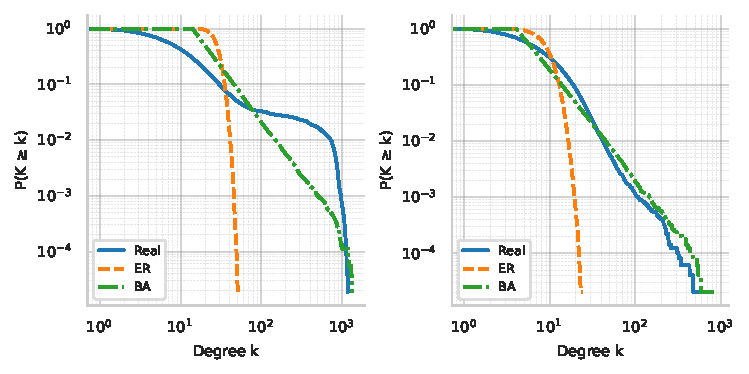
\includegraphics[width=0.9\linewidth]{img/B_degree_ccdf_vs_null.pdf}
\caption{Complementary CDF of degree on a log-log scale for $G_{BC}$ (left) and
$G_{Cit}$ (right), compared against ER and BA null models (dashed).
$G_{BC}$'s tail extends further, consistent with its lower fitted exponent $\hat{\gamma}=2.13$ vs $3.54$.}
\label{fig:degree_null}
\end{figure}

\newpage

\subsection{Centrality Analysis}\label{sec:centrality}
These graph-level properties arise from an uneven distribution of structural roles across nodes. BC's path-shortening effect raises closeness ($\bar{c}$: 0.0870 $\to$ 0.1017); added parallel routes simultaneously dilute betweenness ($\bar{b}$: $2.20 \to 1.69 \times 10^{-4}$, maximum: 0.0666 $\to$ 0.0502). The three measures respond differently at the distributional level (Table~\ref{tab:centrality}): degree and betweenness produce 1\,391 and 970 outliers beyond $\mu+2\sigma$, while closeness yields only 269. Closeness is bounded by global path structure and concentrates in a narrow range (${\approx}0.05$--$0.15$) in both graphs, with no heavy tail.

Rank correlation is moderate to strong ($\rho = 0.78$--$0.85$, Figure~\ref{fig:centrality_all}), yet the top of each ranking is almost entirely reshuffled. Degree overlap at top-10 is zero; closeness reaches just 1/10; even at top-100, both remain negligible (4 and 3 respectively). Betweenness is the exception: 3/10 at top-10 and 44/100 at top-100---key brokers retain their structural role across both graphs. Degree in $G_{BC}$ ranks papers by shared-reference exposure; degree in $G_{Cit}$ by incoming citations---so which graph is analysed determines which collaboration gaps become visible.

\begin{table}[hb]
\centering\footnotesize
\begin{tabular}{@{}lrrrrr@{}}
\toprule
 & Mean & Std & Max & P99 & $>\mu+2\sigma$ \\
\midrule
\multicolumn{6}{@{}l}{\textit{Combined LCC}} \\
\quad Degree      & 27.69   & 103.21  & 1\,169 & 726     & 1\,391 \\
\quad Betweenness & 1.69e-4 & 7.20e-4 & 0.0502 & 2.41e-3 &    970 \\
\quad Closeness   & 0.1017  & 0.0135  & 0.1435 & 0.1263  &    269 \\
\midrule
\multicolumn{6}{@{}l}{\textit{Citation LCC}} \\
\quad Degree      & 8.51    & 10.78   & 621    & 41      & 1\,194 \\
\quad Betweenness & 2.20e-4 & 1.02e-3 & 0.0666 & 3.38e-3 &    857 \\
\quad Closeness   & 0.0870  & 0.0131  & 0.1270 & 0.1107  &    180 \\
\bottomrule
\end{tabular}
\caption{Centrality statistics (NetworKit, undirected LCC) for $G_{BC}$ and $G_{Cit}$. $>\mu+2\sigma$: node count above two std devs.}
\label{tab:centrality}
\end{table}
\begin{figure}[h]
    \centering
    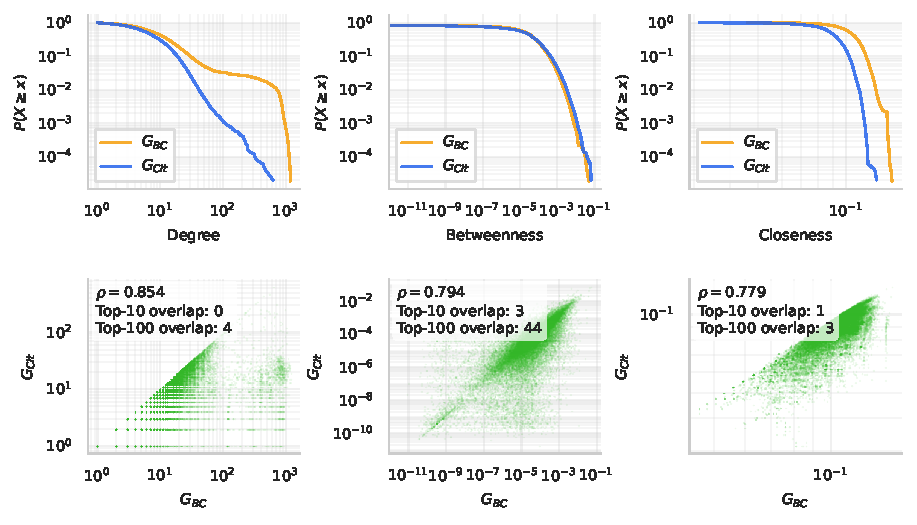
\includegraphics[width=\linewidth]{img/B_centrality_all.pdf}
    \caption{Log-log CCDF (top) and cross-graph scatter with Spearman $\rho$ and top-$k$ overlap (bottom), for degree (left), betweenness (center), and closeness (right).}
    \label{fig:centrality_all}
\end{figure}

\section{Community Detection}
\label{sec:CD}

The topology shifts in Section~\ref{sec:NC}---shorter paths, reshuffled centrality rankings---raise a structural question one level up: do BC's added edges reorganise community membership, and does that reorganisation track disciplinary boundaries?  We run three algorithms on $G_{Cit}$ and $G_{BC}$, validating the resulting partitions against FOS labels at L2 macro-domain and L4 sub-discipline granularity.

\subsection{Ensemble Stabilisation}
\label{subsec:cd:stabilisation}

All three algorithms are stochastic; we stabilise each via an \emph{ensemble-plus-medoid} protocol---run the algorithm $N$ times, compute pairwise NMI across all runs, and select the partition with the highest mean NMI to all others (the medoid).

\begin{itemize}

  \item \textbf{Leiden}~\cite{traag2019louvain} uses \texttt{RBConfiguration}\allowbreak\texttt{VertexPartition}, avoiding the resolution limit of standard modularity~\cite{fortunato2007resolution}.  We sweep $\gamma$ over 30 log-spaced values in $[0.05,\,10]$ with a 100-run ensemble at each point, recording non-trivial community count ($\geq 20$ nodes) in the medoid.  Both graphs show a stable plateau: $\gamma \in [0.05,\,0.578]$ for $G_{Cit}$, $[0.05,\,0.472]$ for $G_{BC}$.  We fix $\gamma_{\text{common}} = 0.154$ from the plateau intersection, trading per-graph optimality for comparability.

  \item \textbf{InfoMap}~\cite{rosvall2008maps} minimises map-equation codelength for a random walker and requires no resolution parameter. $G_{Cit}$ enters as directed and unweighted; $G_{BC}$ as undirected and weighted.  We run a 100-run ensemble and select the medoid.

  \item \textbf{ANGEL}~\cite{rossetti2019exorcising} is the only overlap-aware method.  We calibrate \texttt{threshold} and \texttt{min\_community\_size} by sweeping an $11\times 4$ grid (threshold $\in [0.3,\,0.8]$, min\_size $\in [4,\,7]$) on both graphs and selecting the configuration that best scores coverage, overlap rate, and community count via a composite utility function.  The selected configuration is threshold\,$=0.45$, min\_size\,$=4$.  The ensemble uses 30 runs (reduced from 100: ${\sim}640$\,s per BC run); the medoid is selected via NMI on crisp projections, assigning multi-member nodes to the community containing the most of their neighbours.
\end{itemize}

Table~\ref{tab:cd-summary} confirms that all three methods are stable ($\mu_{\text{NMI}} \geq 0.91$).  InfoMap on $G_{BC}$ shows the widest spread ($\sigma = 0.037$)---the denser graph introduces more flow-routing ambiguity for the random walker.

\subsection{Community Structure and Quality}
\label{subsec:cd:results}

FOS L4 labels cover 44\,317 of 57\,603 nodes ($76.9\%$); the remaining $23.1\%$ introduces uncertainty in any disciplinary classification that follows.  The corpus is biomedical-dominant: medical and health sciences account for $49\%$ of labelled nodes, followed by natural sciences ($36\%$) and engineering ($21\%$; percentages exceed $100\%$ because nodes carry multiple labels).

\begin{table}[t]

  \centering\footnotesize
  \resizebox{\linewidth}{!}{%
  \begin{tabular}{@{}ll cccc cccc@{}}
    \toprule
     & & \multicolumn{4}{c}{Ensemble stability}
       & \multicolumn{4}{c}{Medoid partition} \\
    \cmidrule(lr){3-6}\cmidrule(l){7-10}
    Algorithm & Graph
      & Runs & $\mu_{\text{NMI}}$ & $\sigma$ & Medoid
      & \#Comm. & Med. & Mean & Largest \\
    \midrule
    Leiden  & $G_{Cit}$ & 100 & 0.941 & 0.007 & 0.952 & 1\,533 &  2 & 35.9 &  4\,520 \\
    Leiden  & $G_{BC}$  & 100 & 0.934 & 0.011 & 0.946 & 1\,210 &  2 & 47.6 &  9\,145 \\
    \midrule
    InfoMap & $G_{Cit}$ & 100 & 0.941 & 0.009 & 0.954 & 1\,496 &  3 & 45.7 & 19\,750 \\
    InfoMap & $G_{BC}$  & 100 & 0.910 & 0.037 & 0.934 & 1\,174 &  3 & 55.4 & 22\,940 \\
    \midrule
    ANGEL   & $G_{Cit}$ &  30 & 0.967 & 0.002 & 0.969 & 1\,527 &  9 & 25.4 &  1\,724 \\
    ANGEL   & $G_{BC}$  &  30 & 0.964 & 0.002 & 0.966 & 1\,514 & 10 & 31.3 &  3\,321 \\
    \bottomrule
  \end{tabular}%
  }
    \caption{Ensemble stability and medoid partition statistics.
           $\mu_{\text{NMI}}$: mean pairwise NMI across runs;
           Medoid: that run's mean NMI to all others.
           Leiden: $\gamma = 0.154$; ANGEL: threshold $= 0.45$,
           min\_size $= 4$.  Med.: median community size.}
  \label{tab:cd-summary}
\end{table}

\begin{figure}[t]
  \centering
  \begin{subfigure}[b]{0.15\textwidth}
    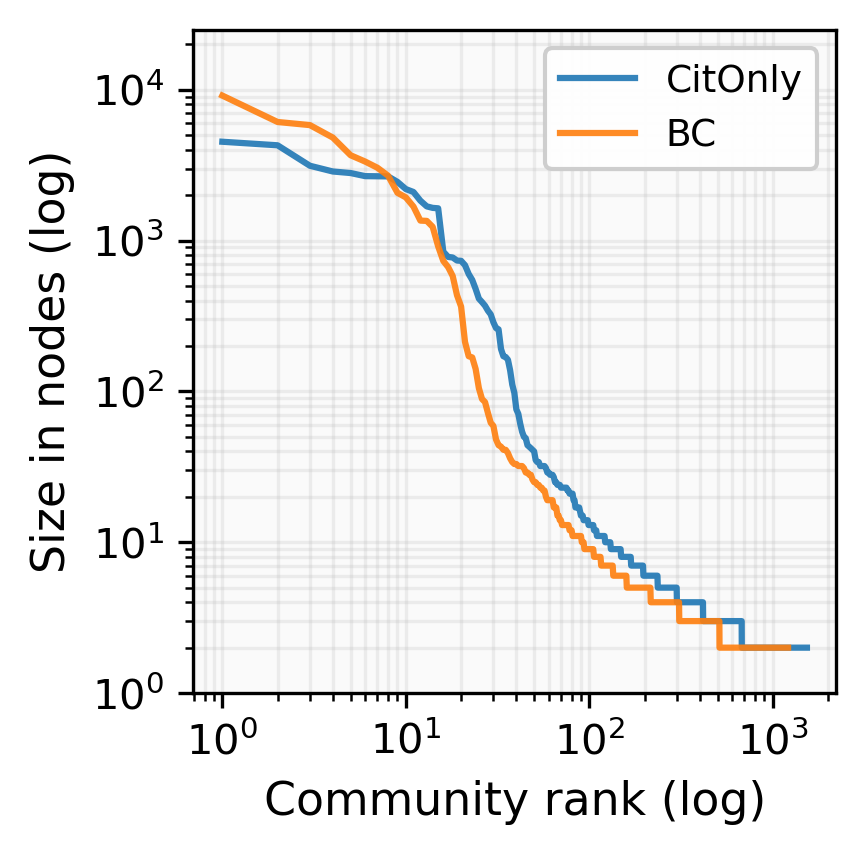
\includegraphics[width=\textwidth]{img/C_leiden_size_distribution.png}
    \caption{Leiden}
    \label{fig:dist-leiden}
  \end{subfigure}
  \hfill
  \begin{subfigure}[b]{0.15\textwidth}
    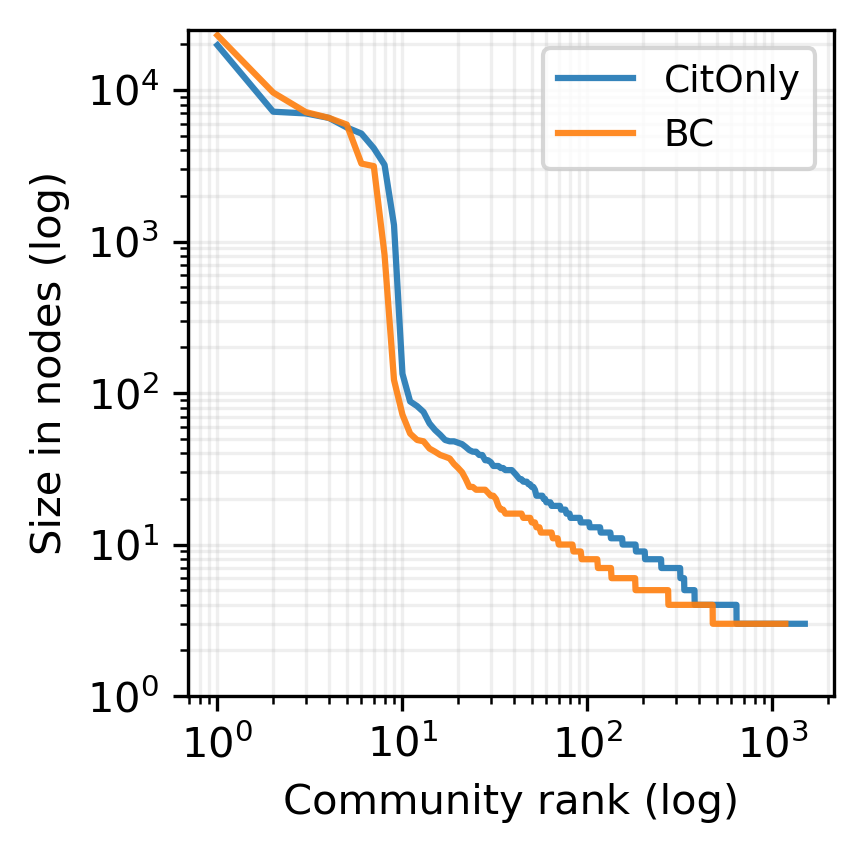
\includegraphics[width=\textwidth]{img/C_infomap_size_distribution.png}
    \caption{InfoMap}
    \label{fig:dist-infomap}
  \end{subfigure}
  \hfill
  \begin{subfigure}[b]{0.15\textwidth}
    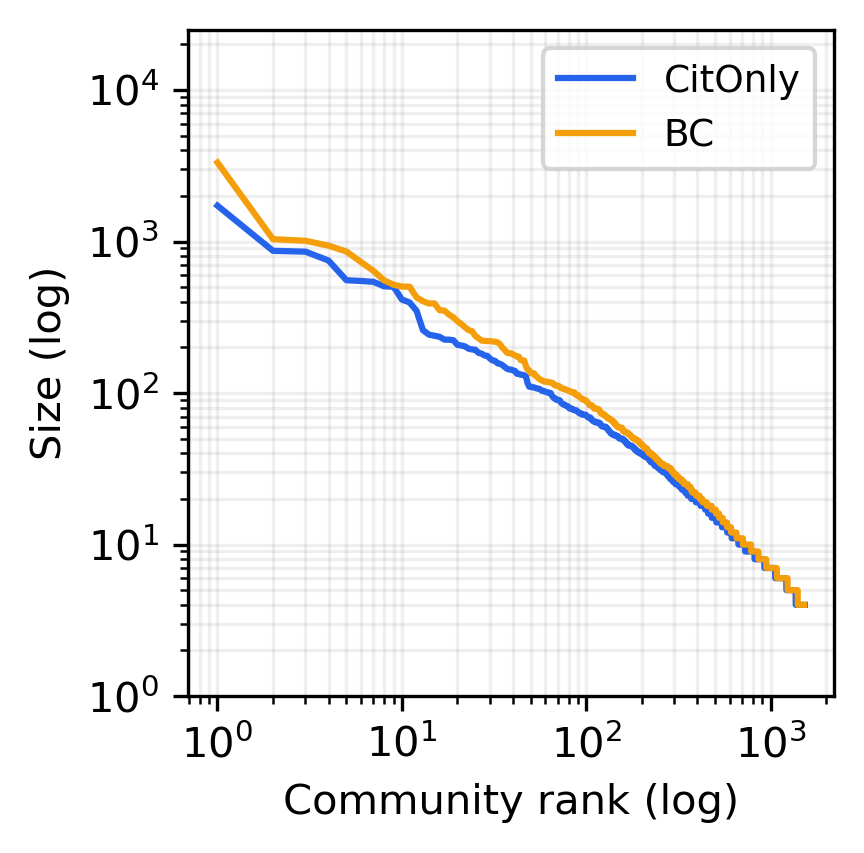
\includegraphics[width=\textwidth]{img/C_angel_size_distribution.png}
    \caption{ANGEL}
    \label{fig:dist-angel}
  \end{subfigure}
  \caption{Community size distributions (medoid partitions).}
  \label{fig:size-dist}
\end{figure}

Leiden and InfoMap agree: BC reduces community count by ${\sim}21\%$ (Table~\ref{tab:cd-summary}).  ANGEL barely moves ($-0.9\%$) because it resolves ambiguity through overlap rather than merging---its largest community nearly doubles ($1\,724 \to 3\,321$), but the total count stays flat.  Median size stays at 2--3 for the crisp methods on both graphs, reflecting the heavy tail typical of citation networks: most communities are tiny and unaffected by BC.  The consolidation happens in the upper tail---Leiden needs 9 communities to cover 50\% of nodes on $G_{Cit}$ but only 5 on $G_{BC}$.

We track what each large $G_{Cit}$ community ($\geq 20$ nodes) becomes on $G_{BC}$.  Leiden registers 18 merge events.  InfoMap concentrates its merges into only 5 events, the largest of which absorbs 10 components into a single community of 19\,664 nodes.  ANGEL stays largely stable (76\%), absorbing change through overlap. Both crisp methods retain measurable modularity on $G_{BC}$ ($Q = 0.681$ for Leiden, $0.597$ for InfoMap)---a substantial drop from $G_{Cit}$ ($Q = 0.939$, $0.837$) that reflects the density tripling, not structural collapse.

At 19\,664 nodes, one InfoMap community covers roughly 36\% of the network; assigning a third of all papers to a single group limits discriminative value regardless of internal coherence.  BC pushes it further to 22\,940 nodes, reinforcing the coarseness already present on $G_{Cit}$.

Semantic purity is measured as normalised Shannon entropy $\hat{H} = H / \log_2 k$ over FOS labels per community ($\geq 10$ nodes); $\hat{H} \to 0$ is pure, $\hat{H} \to 1$ is uniform.  Leiden's L4 entropy rises slightly on $G_{BC}$ ($\bar{H}: 0.612 \to 0.631$)---consistent with cross-disciplinary merges broadening composition. InfoMap moves in the opposite direction ($\bar{H}: 0.683 \to 0.627$), alongside a sharp drop in qualifying communities (182 $\to$ 81)---the partition consolidates rather than diversifies.  Both graphs yield comparable FOS coherence under any given algorithm; BC reshapes community granularity more than disciplinary composition.

\subsection{Cross-Algorithm Synthesis}
\label{subsec:cd:synthesis}

For each of the 18 Leiden merge events (components $\geq 20$ nodes), we check whether InfoMap and ANGEL independently group the same nodes, defining confirmation as $\geq 50\%$ overlap with one community. InfoMap confirms almost every merge (median overlap $\geq 0.98$, both INTRA and CROSS).  ANGEL does not---only 1 of 18 reaches $3/3$ consensus; its median overlap stays at $0.14$ for CROSS and $0.30$ for INTRA, reflecting fragmentation rather than disagreement.  Fifteen of 18 merges ($83\%$) are cross-disciplinary at FOS L4.

To test whether merge zones are more disciplinarily concentrated than their surroundings, we compute Gini impurity $G_I = 1 - \sum_k p_k^2$ and compare it to a multi-hop neighbourhood null (1\,000 permutations).

No merge is testable at hop 1.  Significance emerges at hop 2 (4/7 testable merges, all CROSS) and strengthens at hop 3 (13/16, including the first INTRA).  BC creates structures that become distinguishable from their surroundings only at mesoscopic scale; locally, they blend into the same disciplinary landscape.

A complementary FOS gap analysis counts how often sub-discipline pairs co-occur within the same community in $G_{Cit}$ vs $G_{BC}$.  206 pairs show a positive gap; 55 are entirely new.  But a permutation test (1\,000 shuffles preserving community sizes) finds none significant---all p-values equal $1.000$.
This is the key negative result: the co-occurrence signal is indistinguishable from a random size-preserving partition.


\paragraph{Caveats.}
The $83\%$ CROSS ratio is conditioned on $\gamma = 0.154$, which sits at the lower end of the plateau and produces relatively large communities that span multiple FOS L4 labels \emph{before} any merge, biasing classification toward CROSS.  At higher $\gamma$, the same consolidation would register as more INTRA.  The direction of BC's effect---fewer communities, larger merge zones---is robust across the plateau; the INTRA/CROSS proportion is resolution-dependent, not an absolute structural property.  $23.1\%$ of nodes lack FOS labels; the shared $\gamma_{\text{common}}$ sacrifices per-graph optimality; and ANGEL's 30-run ensemble provides less stabilisation than the other methods, though its tight NMI spread ($\sigma = 0.002$) suggests this is not limiting.
\section{Hypergraph Analysis}\label{sec:HG}

$G_{BC}$ encodes bibliographic coupling as pairwise edges, but projecting to pairs loses a key distinction: when several papers all cite the same external source, the resulting clique in $G_{BC}$ treats every pair as independent, discarding the information that one shared reference mediates all connections. A hypergraph captures this directly. We define $H = (V, \mathcal{E})$ over the UniPi node set; each hyperedge corresponds to one external reference and groups every UniPi paper that cites it. Direct UniPi-to-UniPi citations are excluded, so $H$ isolates the BC signal without duplicating edges already in $G_{BC}$.

$H$ is built from the same citation graph underlying $G_{BC}$ and $G_{Cit}$
(4.86M nodes, 8.27M edges). Restricting to post-2020 UniPi papers, their parent papers, and their shared external references---while discarding external-to-external links---yields a working subgraph of 64,156 UniPi nodes, 3.01M external nodes, and 5.03M edges.

Construction proceeds in three filtering steps. First, for each external reference we collect all connected UniPi papers; references linking fewer than two UniPi papers are discarded, producing 762,800 candidate hyperedges.
Second, multiple references sharing the identical UniPi node-set are collapsed into weighted families, reducing the count to 512,004 unique hyperedges (duplicate rate: 32.9\%; maximum family weight: 1,535). Third, to suppress spurious connections from foundational references cited across many disciplines---a higher-order analogue of the hub problem in pairwise $BC$---we remove the 14 families exceeding 450 UniPi nodes.
Table~\ref{tab:hypergraph_stats} summarises the final structure. Despite a node-degree range spanning three orders of magnitude (median~19, max~6{,}061), the hypergraph is nearly connected: 141 components form, but the LCC absorbs 99.4\% of nodes and only 2 further components reach ${\geq}\,10$ members.

\begin{table}[h]
  \centering
  \footnotesize

  \begin{tabular}{lccc}
    \toprule
                   & \textbf{Median} & \textbf{Mean} & \textbf{Max} \\
    \midrule
    Hyperedge size & 3               & 3.9           & 423          \\
    Node degree    & 19              & 32.2          & 6{,}061      \\
    \midrule
    Hyperedges     & \multicolumn{3}{c}{511,990}                    \\
    Nodes          & \multicolumn{3}{c}{61,369}                     \\
    \bottomrule
  \end{tabular}
    \caption{Descriptive statistics of $H$.}
  \label{tab:hypergraph_stats}
\end{table}

\subsection{S-Line Sensitivity}\label{subsec:hg:sline}

A single shared citation may be coincidental; multiple shared references suggest genuine thematic overlap. The s-line graph $L_s(H)$ tests this directly: it connects two hyperedges whenever they share $\geq s$ nodes, so raising $s$ retains only the densest co-memberships.
Hyperedges with $> 80$ nodes and nodes with hyperdegree $> 300$ are excluded from matrix construction to keep computation tractable, removing 308 nodes and 235 hyperedges and leaving 511,755 working hyperedges over 61,342 nodes.
We track connectivity via the \emph{giant ratio}---the fraction of hyperedges in the LCC of $L_s(H)$---benchmarked against the $G_{Cit}$ LCC baseline of $89.4\%$.

At $s = 1$, the giant ratio is $98.8\%$---nearly the entire hypergraph connects (Table~\ref{tab:sline}). Requiring two shared references drops it to $71.5\%$, already below the $G_{Cit}$ citation baseline: sharing two external sources is more selective than any direct citation link. At $s = 3$ fewer than a third of hyperedges remain in the giant component, and beyond that the structure collapses rapidly.

\begin{table}[h]
  \centering
  \footnotesize
  \begin{tabular}{cccc}
    \toprule
    $s$ & Edges & Components & Giant ratio (\%) \\
    \midrule
     1 & 46{,}442{,}020 &   5{,}966 & 98.8 \\
     2 &  6{,}684{,}734 & 136{,}873 & 71.5$^\dag$ \\
     3 &  1{,}776{,}668 & 337{,}476 & 30.9 \\
     4 &    650{,}389   & 424{,}437 & 13.3 \\
     5 &    290{,}806   & 463{,}630 &  6.0 \\
    \bottomrule
  \end{tabular}
    \caption{S-line graph statistics.
           $^\dag$First threshold below the $G_{Cit}$ LCC baseline
           ($89.4\%$).}
  \label{tab:sline}
\end{table}

\subsection{Gap Candidates and Validation}
\label{subsec:hg:gaps}

A \emph{gap candidate} is a pair of UniPi papers that share $\geq 1$ hyperedge but have no direct citation between them. The overlap matrix yields 2,000,243 such pairs, with a heavy-tailed support distribution: the 90th-percentile support is 4 shared hyperedges, and the top pair shares 1,927.

A node appearing in many hyperedges co-occurs with many partners simply by volume; high-degree nodes dominate raw support rankings regardless of genuine thematic proximity. We debias with the formula
\begin{equation}\label{eq:debias}
  \text{score}_{\text{debias}}(u,v)
  = \frac{|\mathcal{E}_u \cap \mathcal{E}_v|}
         {\sqrt{(d_u + 1)(d_v + 1)}}
\end{equation}
where $d_u$, $d_v$ are citation-graph degrees (missing degrees imputed at the median; $+1$ avoids division by zero for isolated nodes). The correction is severe: Jaccard overlap between the raw and debiased top-30 is 0.111, confirming that without debiasing rankings reflect hub proximity rather than intellectual affinity.

The top debiased pair (score $= 16.73$) shares 417 hyperedges between two clinical medicine papers with mean citation degree 24. Clinical medicine and physical sciences dominate the top 10 (Table~\ref{tab:top-gaps}), consistent with their majority share in the corpus.

\begin{table}[t]
  \centering
  \footnotesize

  \begin{tabular}{cccl}
    \toprule
    Rank & Support & Score & FOS pair \\
    \midrule
     1 &  417 & 16.73 & Clinical med.\ / Clinical med. \\
     2 &  197 & 11.94 & Clinical med.\ / N/A \\
     3 &  163 & 11.30 & Physical sci.\ / Physical sci. \\
     4 &  259 & 11.15 & Clinical med.\ / N/A \\
     5 &  255 & 10.93 & Clinical med.\ / Clinical med. \\
     6 &  211 & 10.35 & Physical sci.\ / Physical sci. \\
     7 &  140 & 10.10 & Physical sci.\ / Physical sci. \\
     8 &  144 &  9.94 & Clinical med.\ / N/A \\
     9 &  171 &  9.78 & Clinical med.\ / N/A \\
    10 &  482 &  9.19 & Physical sci.\ / Physical sci. \\
    \bottomrule
  \end{tabular}
    \caption{Top 10 gap candidates by debiased score. ``Support'' is the number of shared hyperedges; FOS is the L2 domain. N/A indicates unlabelled nodes (23.1\% of the corpus).}
  \label{tab:top-gaps}
\end{table}

Do gap candidates reflect genuine intellectual proximity, or could the same co-occurrence pattern arise from degree structure alone? We test with a degree-preserving null model: \texttt{double\_edge\_swap} on $G_{Cit}$ (200 simulations), measuring citation hit rate for the top 2,000 pairs by raw hyperedge support.
The observed hit rate is 69.1\%, against a null mean of 1.3\% ($\pm 0.24\%$), yielding $z = 284.5$ ($p < 0.01$). Shared external references predict citation at $55{\times}$ the null rate; the signal survives a degree-preserving stress test and cannot be attributed to hub nodes or degree heterogeneity.


\subsection{Characterisation of Top Gap Candidates}
\label{subsec:hg:characterisation}

For each of the top 100 debiased gap candidates, we check two conditions against the Leiden partitions: (1) whether both nodes changed community assignment between $G_{Cit}$ and $G_{BC}$ (merge zone), and (2) whether both land in the same Leiden community on $G_{BC}$. 92\% of top-100 gap candidates share the same Leiden community on $G_{BC}$, against a random baseline of 0.3\%.
The merge-zone statistic is uninformative: membership is universal among both gap candidates and random pairs at $\gamma = 0.154$, where community reassignment is too pervasive to discriminate. The same-community convergence is therefore the stronger signal: two independent representations---pairwise BC communities and hyperedge co-occurrence---place the same paper pairs together without having been designed to agree.

Of the top 50 debiased gap candidates, 36 (72\%) connect papers in the same FOS L2 domain, and 38 (76\%) share at least one L2 domain (the difference arises because FOS labels are multi-valued and a paper may carry more than one L2 tag). The frequency of unlabelled nodes among top pairs is consistent with their base rate in the corpus (23.1\%), suggesting no systematic bias
toward unclassified papers. Twelve pairs (24\%) span different domains entirely---the candidates that no within-domain search strategy would surface.
The dominance of same-domain pairs is consistent with the community-detection finding that BC primarily consolidates intra-disciplinary fragments (Section~\ref{sec:CD}); cross-domain co-occurrence emerges only through the hypergraph.


\paragraph{Limitations.}
The highest-connected structures are precisely where cross-disciplinary overlap is most likely to appear, and both computational thresholds remove them: hyperedges with $> 80$ nodes from overlap computation, nodes with hyperdegree $> 300$ from s-line construction. Raw support counts shared reference occurrences: widely-cited methodological papers inflate co-occurrence even after hub filtering, and the debiasing corrects for citation-graph degree but not for reference-list heterogeneity.
The null model validates citation prediction, not research fit: shared references establish thematic proximity, not that collaboration would be productive---an inference that requires domain expertise the network cannot supply.
\section{Latent Intellectual Communities in a Research Institution}
\label{sec:Q}
Does a research institution harbour latent intellectual communities whose members work on related problems without directly engaging with each other's work---and can such communities be surfaced from publication records alone?

Citation is a selective and socially shaped practice: researchers cite work they know, and knowledge often travels within established collaboration networks rather than across them. Furthermore, institutional boundaries do not automatically generate awareness: two groups within the same university may develop parallel research programmes in isolation, connected only through shared reference pools rather than through direct intellectual exchange. When both phenomena operate simultaneously, the citation graph will systematically underrepresent the true intellectual proximity within the institution.

\subsection{BC-corrected communities and localisation of gaps}
\label{subsec:q:bccorr}

We started from structural convergence: if hyperedge co-occurrence and bibliographic coupling capture the same latent signal, gap candidates should localise in precisely those communities that BC \emph{corrects}---communities that appear disconnected under pure citation but merge when external references are added.

On $G_\text{CitOnly}$, the three algorithms produce approximately the same number of communities (with different properties and characteristics; see \ref{sec:CD}), but the $G_\text{BC}$ effect diverges across algorithms, each fusing a different share of communities (Table~\ref{tab:bccorr}). 

% TODO – CONTESTO MANCANTE
% Questa frase apre il risultato principale di Sezione 6 ma risulta decontestualizzata. Prima di essa occorre:
%   1. Ricordare brevemente la distinzione fused/stable (definita in Sec. 4)
%   2. Motivare la scelta di top-200 (vs top-100 usato in Table 9)
%   3. Aggiungere una frase di transizione tipo:
%      "To test whether gap candidates localise in structurally corrected regions of the graph, for each of the 200 top-ranked debiased gap candidates (Section 5) we record..."
% In alternativa, spostare la definizione di fused/stable in un mini-reminder inline: "...fused community (one in which BC merged two or more G_{CitOnly} communities) or a stable one (unchanged by BC)..."

To test whether gap candidates localise in structurally corrected regions of the graph, for each of the 200 top-ranked debiased gap candidates obtained in Hypeergraph analysis (Section 5) we record whether its two nodes land in the same $G_\text{BC}$ community, and whether that community is \textbf{fused} (one in which BC merged two or more $G_\text{CitOnly}$ communities) or \textbf{stable} (membership unchanged by BC).

\begin{table}[h]
\centering
\begin{tabular}{lccc}
\toprule
Algorithm & G$_\text{CitOnly}$ comms & Fused comms \\
\midrule
Leiden & 1\,533 & 68   \\
InfoMap & 1\,496 & 46   \\
ANGEL (crisp) & 1\,526 & 355  \\
\bottomrule
\end{tabular}
\smallskip
\caption{Fused communities in $G_\text{BC}$. For ANGEL, any $G_\text{CitOnly}$ community in an overlap counts as fused; the higher count reflects boundary sensitivity rather than structural change.}
\label{tab:bccorr}
\end{table}


All 200/200 gap candidates fall in fused communities---a design consistency check rather than a discovery: no candidate drifts into the 7.6\% of nodes where BC leaves the partition unchanged, which would signal a malfunction of the scoring function.

The interpretation is structural: BC and the hypergraph converge on the same latent communities at two different scales.  BC (macro level) identifies where citation has \emph{fragmented} an intellectually coherent group---the 68 fused communities.  The hypergraph (micro level) identifies \emph{which specific pairs} within those corrected groups share references without citing each other.  %[REVISED: removed redundant tail clause that restated the preceding independent clause]
The 930 stable communities produce zero gap candidates: citation had already drawn those boundaries correctly.

The remaining analyses (§§\ref{subsec:q:conv}--\ref{subsec:q:neardup}) use the top-100 shortlist, the subset subjected to manual title inspection, topic classification, and temporal analysis.  The full top-200 pool serves only the automated BC-localisation check above; rank-band validation (\S\ref{subsec:q:conv}) confirms same-community rates of 100\% for ranks~1--150 and 96\% for ranks~151--200, validating top-100 as the high-confidence working set.

\subsection{Cross-Algorithm Convergence}
\label{subsec:q:conv}
For each of the top~100 debiased gap candidates we check whether both
nodes belong to the same community under each of the four
algorithm-graph configurations.  Figure~\ref{fig:cross_algo}
reports the results alongside random baselines computed over 2\,000
uniformly sampled uncited node pairs.

The Leiden $G_\text{CitOnly}$ control already reaches 99\%---hyperedge
co-occurrence is itself a strong intra-community signal, independent of
BC restructuring.  Adding BC edges lifts Leiden to 100\%; InfoMap and
ANGEL both confirm 100\%.

The enrichment factor varies by two orders of magnitude---from
$5.3\times$ (InfoMap) to $83.3\times$ (ANGEL)---reflecting differences
in partition granularity, not in the underlying signal.  InfoMap's high
baseline (18.8\%) is a consequence of the $\approx$23\,000-node
super-community identified in Section~\ref{sec:CD}.  ANGEL, which
distributes ambiguous nodes across multiple communities, yields the
cleanest enrichment because its crisp projection produces many small
communities (median size~10 on~$G_\text{BC}$) and thus a very low
baseline.

Bootstrap validation (2,000 draws of 100 random uncited pairs, Leiden)
gives a null mean of 7.2\%, never exceeding 16\%; gap candidates achieve
100\% ($p < 0.0005$, minimum reportable with 2,000 replicates).
Stratifying by rank band, the same-community rate is stable: 100\% for
ranks~1--150 and 96\% for ranks~151--200.

\begin{figure}[t]
\centering
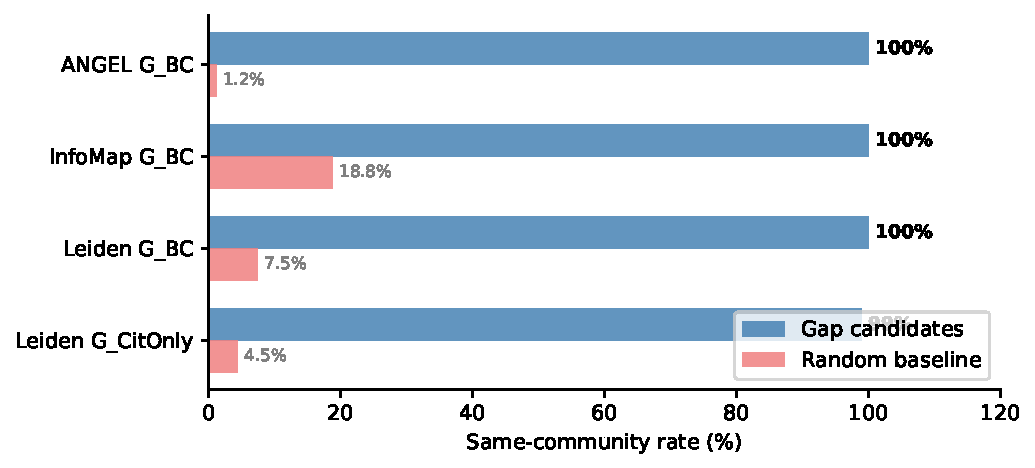
\includegraphics[width=0.45\textwidth]{img/cross_algo_robustness.pdf}
\caption{Same-community rate for the top-100 gap candidates vs.\ random
baseline (fraction of random uncited pairs sharing a community), under
four algorithm-graph configurations.  The $G_\text{CitOnly}$ bar is the
no-BC control.}
\label{fig:cross_algo}
\end{figure}

%-----------------------------------------------------------------------
\subsection{Disciplinary and Thematic Profile of Gap Candidates}
\label{subsec:q:discip}
%-----------------------------------------------------------------------

%[REVISED: merged §Topic Cluster Analysis into §Disciplinary Identity; subsection header eliminated; opening trimmed; LLM sentence dissolved into topic paragraph as transition]
Despite spanning 55\,078 UniPi nodes, the 100 top gap candidates
concentrate in only 6 of the 1\,210 $G_\text{BC}$ communities
(Figure~\ref{fig:community_profile}).  Five exhibit at least 60\%
FOS~L4 sub-discipline purity; the sixth (C3, Chemical sciences)
reaches only 45\% (Table~\ref{tab:comms}).  At the pair level, 81 of
100 share the same four-digit FOS code; the remaining~19 lack a tag on
one side but are confirmed same-topic by title
inspection---consistent with the finding in Section~\ref{sec:HG} that
72\% of the top-50 gap candidates share an FOS~L2 domain.

\begin{table}[h]
\centering
\small
\begin{tabular}{lrrll}
\toprule
C & Size & Gap pairs & Dominant FOS~L4 & Purity \\
\midrule
C8  & 2\,074 & 53 & 0103 Physical sciences  & 79\% \\
C0  & 9\,145 & 30 & 0302 Clinical medicine  & 60\% \\
C7  & 2\,693 & 10 & 0103 Physical sciences  & 60\% \\
C5  & 3\,340 &  4 & 0302 Clinical medicine  & 64\% \\
C3  & 4\,817 &  2 & 0104 Chemical sciences  & 45\% \\
C11 & 1\,356 &  1 & 0103 Physical sciences  & 68\% \\
\bottomrule
\end{tabular}
\caption{$G_\text{BC}$ communities (Leiden) hosting gap candidates.
Purity = fraction of nodes sharing the dominant FOS~L4 sub-discipline.}
\label{tab:comms}
\end{table}

Title-level classification by an LLM (Claude Opus 4.6), verified by
manual inspection,\footnote{Standard text-clustering pipelines
(TF-IDF, BERTopic) were inadequate on this dataset: OpenAIRE keyword
fields are sparsely populated and inconsistently formatted, producing
degenerate clusters.  LLM-assisted classification was adopted as a
pragmatic alternative.} confirms 95 genuine gap pairs among the
top-100 candidates (5 near-duplicates; see
Section~\ref{subsec:q:neardup}).  The two dominant clusters are
gravitational-wave and astrophysics research (47 pairs, 33 unique
UniPi nodes, publications spanning 2010--2024) and
diabetes/cardiovascular medicine (18 pairs).  Smaller clusters cover
HEP/particle physics (9~pairs), thyroid and endocrine disorders (5),
and oncology (4); the remainder spans vascular surgery, rheumatology,
and 8~pairs without a domain label (Figure~\ref{fig:topic_clusters}).

\begin{figure}[t]
\centering
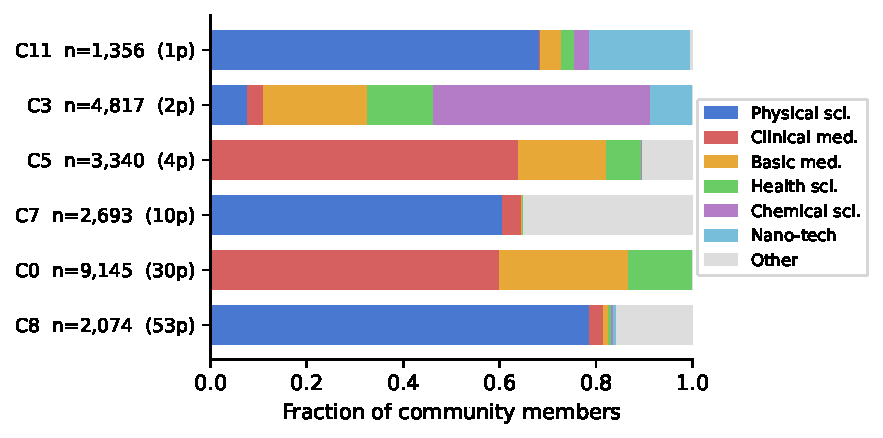
\includegraphics[width=0.45\textwidth]{img/community_fos_profile.pdf}
\caption{Disciplinary composition of the 6 $G_\text{BC}$ communities
hosting gap candidates (Leiden).}
\label{fig:community_profile}
\end{figure}

The GW/astrophysics cluster is the clearest example of a
\emph{citation-invisible} community that the pipeline recovers from
bibliographic records alone---and thereby validates its own
sensitivity.  Thirty-three UniPi nodes contribute to the Einstein
Telescope and LIGO/Virgo collaborations: they share dense reference
overlap, publish in overlapping venues, and work on the same detector
physics.  In mega-collaborations of this scale, researchers co-author
experiment-wide papers and share data pipelines; the members know each
other, so their proximity is not sociologically latent. It is,
however, \emph{invisible in the internal citation graph}: cross-unit
citation is not how collaborative output is recorded.  The GW case
thus serves as a \emph{positive control}: a community whose existence
is independently known and that the pipeline correctly identifies.
The diabetes/cardiovascular and HEP clusters (18 and 9~pairs
respectively), where researchers are less likely to know each other
through shared collaboration structures, are stronger candidates for
the ``latent'' label.
\begin{figure}[h]
\centering
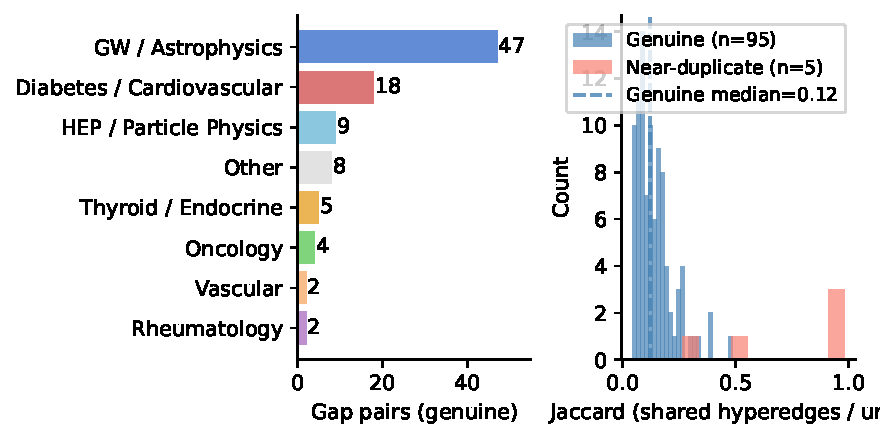
\includegraphics[width=0.45\textwidth]{img/topic_clusters.pdf}
\caption{Distribution of the 95 genuine gap pairs across topic clusters.}
\label{fig:topic_clusters}
\end{figure}

\subsection{What Bibliographic Coupling Adds to the Hyperedge Signal}
\label{subsec:q:hevsbc}

An ablation study compares the top-50 gap candidates produced by three
scoring regimes on the same graph: (A)~hyperedge-debiased
score~\eqref{eq:debias} alone; (B)~BC-weight score alone (raw
bibliographic-coupling edge weight, no degree correction); and (C)~the
full combined pipeline.  The overlap between regimes~A and~B is zero:
$|\text{top-50}_A \cap \text{top-50}_B| = 0$.

Regime~B without degree correction is dominated by pairs with BC-weight
exactly~1.0 and degree~$\approx 1.3$---supplementary files of the same
paper, which share a single external reference and have virtually no
other connections.  These are artefacts of document fragmentation in
the OpenAIRE metadata, not collaboration gaps.  Regime~A, by contrast,
surfaces pairs with mean degree~$\approx 53$ and a mean of 344 shared
hyperedges---papers well-embedded in the citation network with a broad
reference context.

%[REVISED: two conflated facts (A∩C and B∩C) separated into explicit statements; inline formula removed and replaced with prose]
Regimes~A and~C share 47 of their respective top-50 pairs, confirming that HE-debiased scoring drives the combined pipeline. Regime~B contributes none of those top-50: its candidates are entirely displaced by artefacts and do not survive into the combined ranking.  BC's contribution is structural rather than ranking-based: BC-corrected community assignments provide the localisation context within which HE-ranked pairs are validated.  HE identifies \emph{which} pairs share thematic context; BC identifies \emph{where} in the community structure those pairs sit.

\subsection{Temporal Structure of Gap Candidates}
\label{subsec:q:temporal}

The 100 gap candidates distribute across three temporal categories:
69~pairs in which both nodes were published before 2020
(\emph{Parent--Parent}), 22~pairs in which one node is recent
($\geq 2020$) and the other is not (\emph{Recent--Parent}), and
9~pairs in which both nodes are recent (\emph{Recent--Recent}).
The median year gap within a pair is 2~years (mean~3.3, max~13);
18~pairs share the same publication year.  Spearman
$\rho(\text{score},\,\text{year gap}) = -0.14$ ($p = 0.16$,
n.s.)---the gap score is not biased toward temporally distant pairs.

The dominant gap type is not ``two contemporaneous researchers who are
unaware of each other'' but rather ``two papers---often from different
UniPi generations---that share intellectual context without direct
citation.''  For operational purposes, the 9~Recent--Recent pairs
carry the strongest collaboration plausibility; applying the
near-duplicate filter (Section~\ref{subsec:q:neardup}) reduces this
to 7~genuine pairs: 6 within the GW/astrophysics community and
1~HEP pair (score~$= 7.58$, Jaccard~$= 0.49$) representing two
particle-physics groups sharing a broad reference context without
any direct citation.  The 22~Recent--Parent pairs may identify cases
where a current researcher has not cited a still-active older
colleague.  The 69~Parent--Parent pairs document historical thematic
proximity with limited immediate actionability.


\subsection{Near-Duplicate Detection}
\label{subsec:q:neardup}

Among the top-100 candidates, 3 pairs are removed by a Jaccard
similarity threshold of $\geq 0.70$ on their shared-hyperedge sets;
2 further pairs, with $J = 0.265$ and $J = 0.520$, are flagged by
manual inspection as same-paper duplicates published in different
venues (e.g., an ESC consensus statement appearing in two journals,
or a LIGO paper appearing as both a preprint and a journal article).
All 5 are excluded from the topic and temporal analyses above and
flagged in the exported candidate list as a sensitivity signal.

These cases survive OpenAIRE deduplication~\cite{openaire_dedup},
which does not resolve deliberate multi-venue publications where
records are genuinely distinct in provenance.  A production deployment
would benefit from a pre-filter based on title similarity or DOI
crosswalk, applied \emph{before} hyperedge construction.

\section{Conclusions and Limitations}
\label{subsec:q:scope}

\paragraph{Answer to the research question.}
Yes: the institution does harbour latent intellectual communities
recoverable from publication records alone.  The strongest evidence
is the GW/astrophysics group---33 UniPi researchers whose shared
intellectual context is invisible in the citation graph but fully
legible in shared external references.  More broadly, all 200 gap
candidates localise in BC-corrected communities, concentrate in 6
disciplinarily coherent communities (FOS~L4 purity $\geq 45\%$,
five of six $\geq 60\%$), and are confirmed across three algorithms
and a bootstrap null ($p < 0.0005$).

\paragraph{What the evidence does not show.}

\textit{No ground truth.}  The analysis is entirely structural:
thematic proximity and community coherence are necessary but not
sufficient to confirm a missed collaboration.

\textit{Temporal actionability is limited.}  Sixty-nine per cent of
candidates pair two pre-2020 papers, documenting historical proximity
rather than current opportunity.  The 9~Recent--Recent pairs are the
operationally relevant subset.

\textit{Within-discipline scope.}  The pipeline operates within
FOS~L4 sub-disciplines at the current debiasing threshold;
cross-disciplinary gap detection would require a different scoring
function.

\paragraph{Directions for enhancement.}
The pipeline identifies \emph{where to look}; three targeted
enhancements would convert its output into actionable
recommendations.  \textit{Temporal filtering}---restricting
candidates to Recent--Recent pairs---eliminates the 69\% reflecting
historical accumulation as a one-line filter on existing output.
\textit{Author-level lifting} (nodes = researchers, edges =
co-authorship or co-citation via ORCID) would enable recommendations
of the form ``researcher $X$ and researcher $Y$ share 15 reference
clusters but have never co-authored''---contingent on disambiguation
coverage.  \textit{Retrospective validation}---flagging 2020
candidates and checking for co-authorship by 2025---would yield the
first empirical precision and recall estimates for BC-based
collaboration prediction at the institutional level.  The
7~genuine Recent--Recent pairs identified in
Section~\ref{subsec:q:temporal} are the natural starting point: few
enough for manual review, recent enough to be actionable, and robust
across all three algorithms.

\textit{Multi-hop proximity.}  Both components measure affinity at the
first hop only: shared direct references (HE) or shared direct
citation neighbours (BC).  Extending to second-order
metrics---bibliographic coupling on the hypergraph, personalized
PageRank on the citation graph---would capture transitive proximity
currently invisible to the scoring function.

\bibliographystyle{ACM-Reference-Format}
\bibliography{biblio}

\end{document}